% !TEX root = ../../main.tex
\begin{figure*}[p!]
  \centering
%  \pdfimageresolution=500
  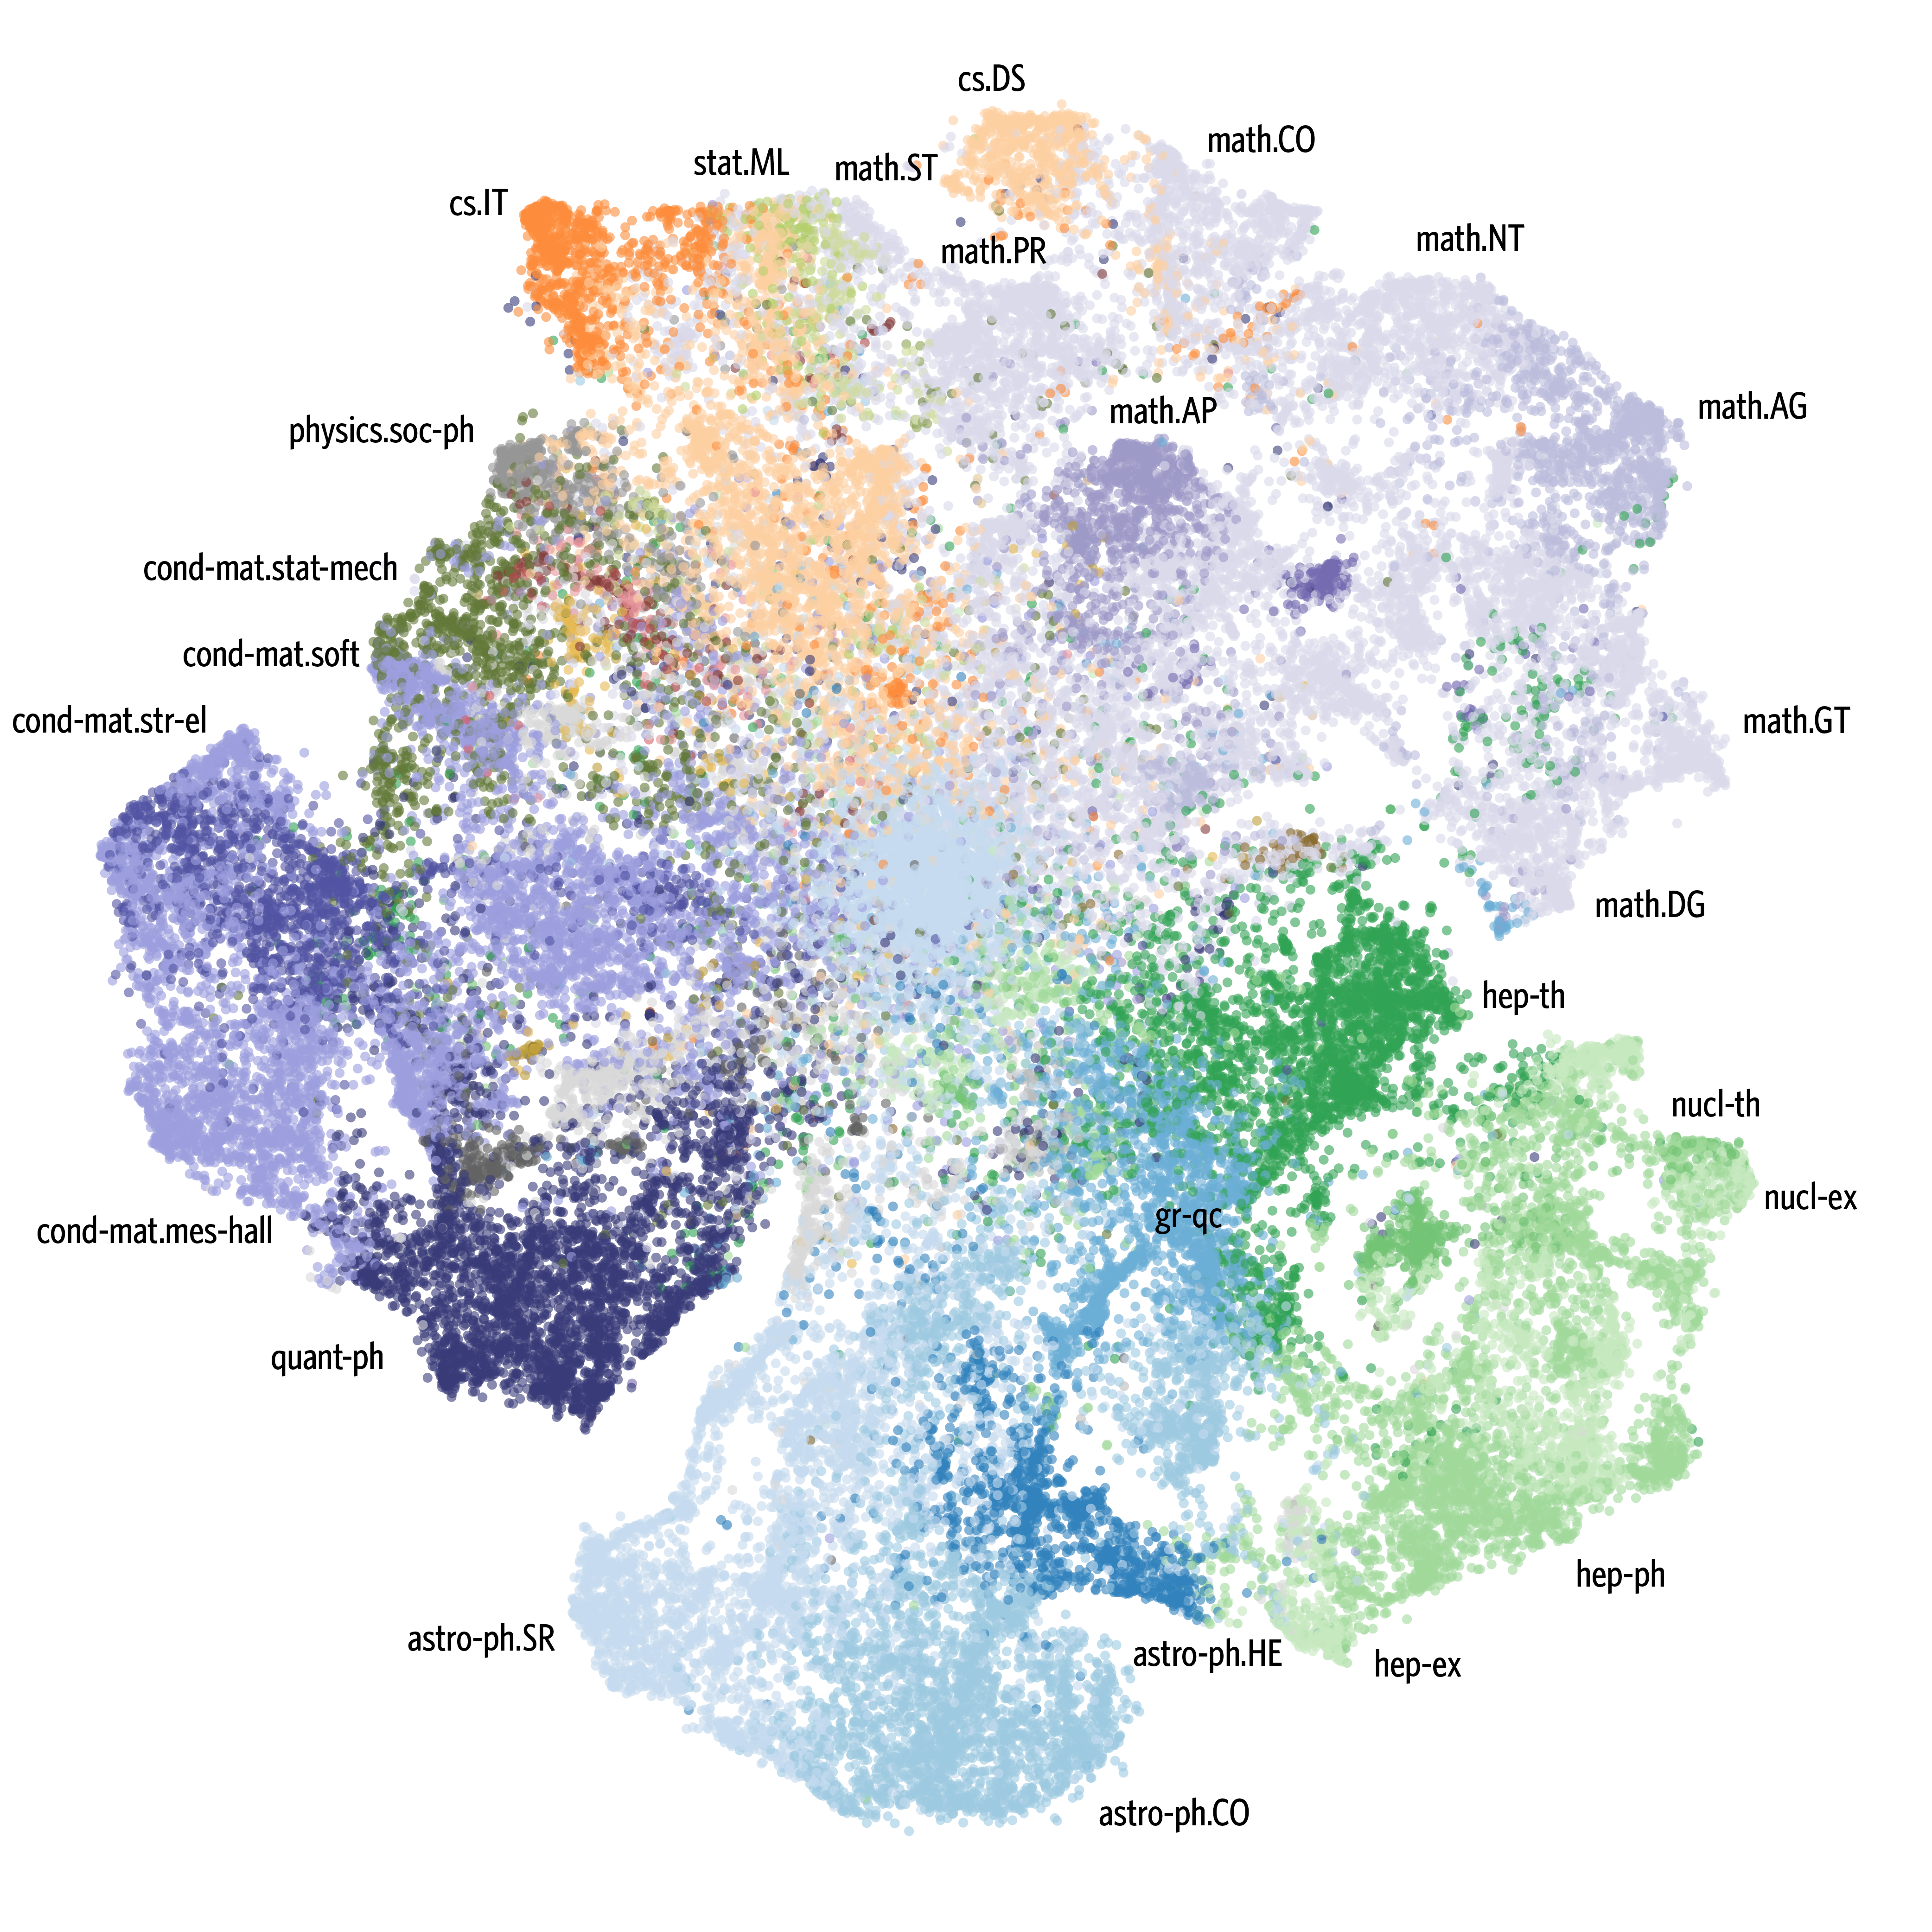
\includegraphics[width=1.0\textwidth]{ch-rfs/fig/arxiv_user_embeddings_tsne.png}
  \caption[Qualitative evaluation of \textsc{rfs} on arXiv reading behavior data]{\label{fig:arxiv_tsne} \textbf{\acrlong{rfs} trained on arXiv reading behavior clusters researchers by their most frequently-read arXiv category (best viewed on a screen).} \gls{rfs} is trained to recommend items using their attributes (words in the abstract). t-SNE~\citep{maaten2008visualizing} is used to visualize the user embeddings $\theta_u$ in the inner product regression function in \Cref{eqn:rankfromsets}. Each marker represents a user embedding; its color represents a user's most-read arXiv category. Unique colors are determined using the most-read categories across the arXiv, and colors are assigned according to the arXiv ontology. \gls{rfs} captures usage patterns, as fields of study are related by patterns of reading behavior across neighboring fields (e.g. \texttt{stat.ML} and \texttt{cs.IT}).} %An interactive map with all labels can be accessed at %\href{http://j.mp/rankfromsets}{\texttt{http://j.mp/rankfromsets}}.}
\end{figure*}
\clearpage